\section{Results}
\subsection{Plaquette expectation value}
As first comparison and comfirmation of our setupt, we will calculate the plaquette expectation value. It is definied as the following:
\begin{align}
	\Braket{P} = \Braket{\sum_{\vec{r}}\frac{P_{\vec{r}}+P_{\vec{r}}^{\dag}}{2}}.
\end{align}
From the scaling of the Hamiltonian in respect to $g$ we would expect $\lim_{g\rightarrow\infty}\Braket{P}=0$ and $\lim_{g\rightarrow0}\Braket{P}=1$. \cref{fig:2exp} is the result of the calculation and as we see, it behaves as expected. % TODO: what does the exp value mean intuitivly? (percentage contribution to the hamiltonian) 
\begin{figure}[h]
	\begin{center}
		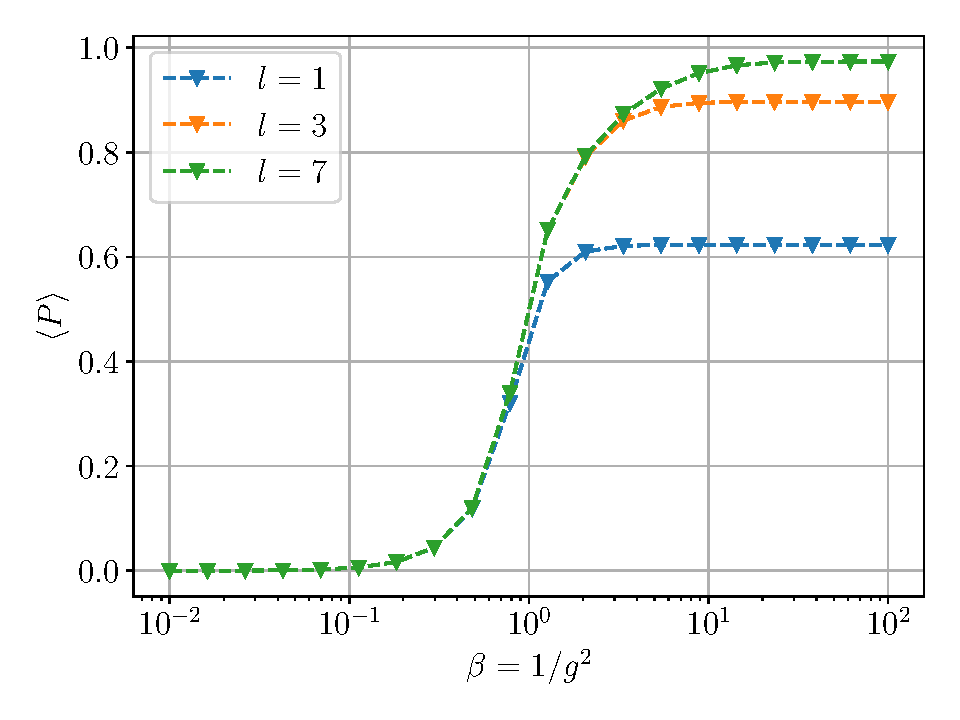
\includegraphics[width=0.45\textwidth]{images/PlaquetteExp2x2PBC.pdf}
	\end{center}
	\caption{plaquette expectation values for a $2\cross2$ lattice with PBC.}\label{fig:2exp}
\end{figure}
An interesing but not suprising observation is the convergance of the expectation value to 1 for large $\beta$ with the order of truncation. Thus using large $l$ is favourable.

As a next step we look at the next larger lattice and use dimensions of $3\cross3$. \cref{fig:3exp} shows the results. Here we want to focus only on larger $\beta$.
\begin{figure}[h]
	\begin{center}
		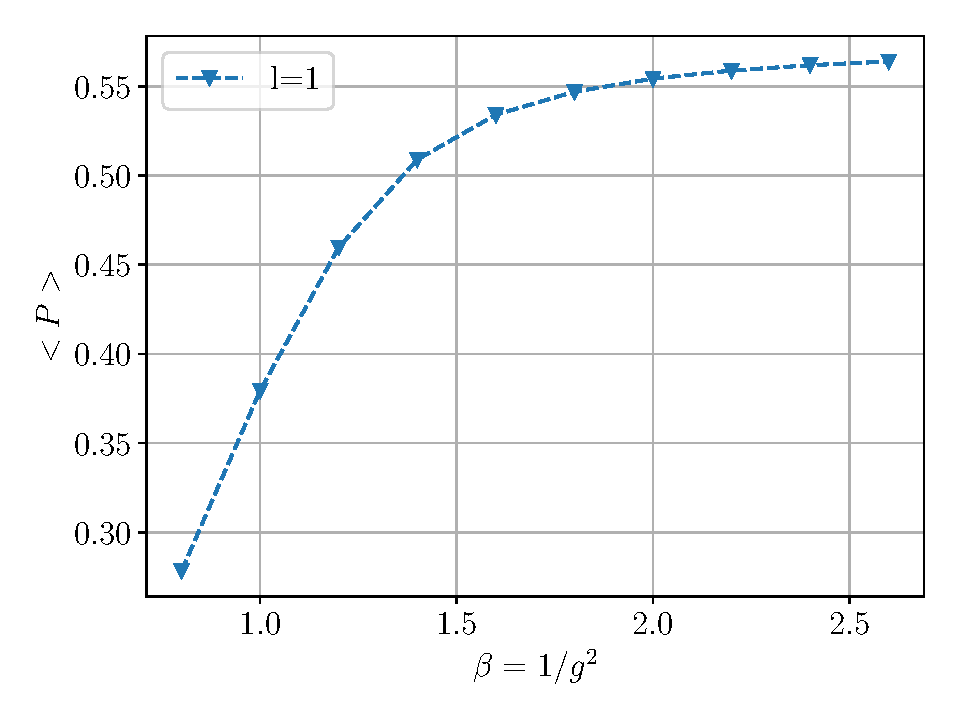
\includegraphics[width=0.45\textwidth]{images/PlaquetteExp3x3PBC.pdf}
	\end{center}
	\caption{Plaquette expectation values for a $3\cross3$ lattice with PBC.}\label{fig:3exp}
\end{figure}
\newpage
Here we can also confirm the convergence to 1 as we increase $\beta$ and the truncation. Especially this Figure and its results are direcetly comparable to the figure from Arianna Crippa et al. (2024)\cite{crippa2024}


\subsection{Quark-Antiquark potential}
Now for calculating the quark antiquark potential we need to subtract the energy of the chargeless lattice $H_{0}$:
\begin{align}
	V = \Braket{H} - \Braket{H_{0}}
\end{align}
with $H$ beeing the lattice with the desired charge. For our porpose we place one charge in the buttom left corner and place the opposite charge at a lattice site with desired distance. We also want to study the effect of diffrent setups on charge pairs with the same distance. Thus we will vary the truncation $l$ from 1 to 3 and also compare the orginal $3 \cross 3$ lattice with no PBC with a lattice with PBC and a lattice with dimensions $4\cross 4$. With these diffrent setups we optain \cref{fig:qqbar}. Throughout this section this is the central Figure, that we will discuss.
\begin{figure}[h]
	\begin{center}
		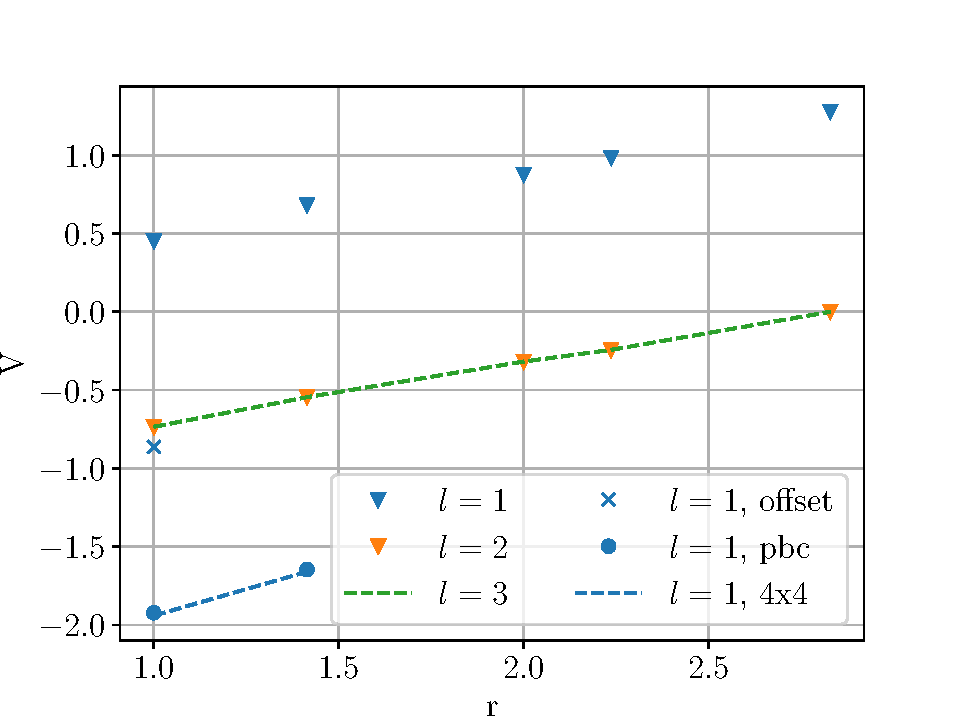
\includegraphics[width=0.45\textwidth]{images/quark_antiquark_potential_normal_g.pdf}
	\end{center}
  \caption{Quark-Antiquark potential for diffrent but comparable setups at $g=\num{1}$. By default $3\cross3$ dimensions and no PBC, if not stated otherwise.}\label{fig:qqbar}
\end{figure}
Firstly we take a look at most basic setup: A $3\cross 3$ lattice with no PBC and a trancation of $l=1$. Here we can see the basic behaviour for increasing distance $r$. The potential raises, which hints that we experience confienemnt. %TODO: More explanation

Now we watch what happens if we vary diffrent lattice parameters. If we choose a diffrent truncation $l$, here 2 and 3, the potential has the same behaviour but is negativly shifted. This is to be expected, since as we approach continuum, and the lattice fragments vanish, we also approach the true lowest energie eigenstate. We also see, that the diffrence from $l=1$ to $l=2$ is quite signifacant, but the next stept, from $l=2$ to $l=3$, is barely notacable. This shows, that that a truncation of at least $l=2$ is favourable.

For the next comparison we watch what happens if we do not set the charge pair at the rim, but at the center. We would also expect a negative shift of the potential, since at the rim we would never see the translational invariance of the continuum. Only at the center we could get an approximate translational invariance. The scene is sketched in \cref{fig:3x3no}. The normal setup is used for our initial calculation with $l=1$ at $r=1$ (upside down triangle). The potential of the offset setup is now depicted by the blue cross in \cref{fig:qqbar}. We can see that indeed the potential also gets a negative shift. An interesting side note is that it shifts even further then the improvement in truncation.
\begin{figure}[h]
	\begin{center}
		
\subfloat[normal]{
	\begin{tikzpicture}[thick,decoration={
					markings,
					mark=at position 0.5 with {\arrow{>}}}
		]

		\tikzset{
			site/.style={
					circle, draw=gray, fill=gray!20, line width=1.5pt, inner sep=0pt, outer sep=4pt, minimum size=0.4cm
				},
			pcharge/.style={
					circle, draw=red, fill=red!20, line width=1.5pt, inner sep=0pt, outer sep=4pt, minimum size=0.4cm
				},
			ncharge/.style={
					circle, draw=blue, fill=blue!20, line width=1.5pt, inner sep=0pt, outer sep=4pt, minimum size=0.4cm
				},
		}
		\node[pcharge](s1){\textbf{$+$}};
		\node[site, right=0.8cm of s1](s2){};
		\node[site, right=0.8cm of s2](s3){};
		\node[ncharge, above=0.8cm of s1](s4){\textbf{-}};
		\node[site, above=0.8cm of s2](s5){};
		\node[site, above=0.8cm of s3](s6){};
		\node[site, above=0.8cm of s4](s7){};
		\node[site, above=0.8cm of s5](s8){};
		\node[site, above=0.8cm of s6](s9){};


		\draw[postaction={decorate}] (s1)--(s2);
		\draw[postaction={decorate}] (s2)--(s3);

		\draw[postaction={decorate}] (s1)--(s4);
		\draw[postaction={decorate}] (s2)--(s5);
		\draw[postaction={decorate}] (s3)--(s6);

		\draw[postaction={decorate}] (s4)--(s5);
		\draw[postaction={decorate}] (s5)--(s6);

		\draw[postaction={decorate}] (s4)--(s7);
		\draw[postaction={decorate}] (s5)--(s8);
		\draw[postaction={decorate}] (s6)--(s9);

		\draw[postaction={decorate}] (s7)--(s8);
		\draw[postaction={decorate}] (s8)--(s9);

	\end{tikzpicture}
}
\hspace{0.01\textwidth}
\subfloat[offset]{
	\begin{tikzpicture}[thick,decoration={
					markings,
					mark=at position 0.5 with {\arrow{>}}}
		]

		\tikzset{
			site/.style={
					circle, draw=gray, fill=gray!20, line width=1.5pt, inner sep=0pt, outer sep=4pt, minimum size=0.4cm
				},
			pcharge/.style={
					circle, draw=red, fill=red!20, line width=1.5pt, inner sep=0pt, outer sep=4pt, minimum size=0.4cm
				},
			ncharge/.style={
					circle, draw=blue, fill=blue!20, line width=1.5pt, inner sep=0pt, outer sep=4pt, minimum size=0.4cm
				},
		}
		\node[site](s1){};
		\node[pcharge, right=0.8cm of s1](s2){\textbf{$+$}};
		\node[site, right=0.8cm of s2](s3){};
		\node[site, above=0.8cm of s1](s4){};
		\node[ncharge, above=0.8cm of s2](s5){\textbf{-}};
		\node[site, above=0.8cm of s3](s6){};
		\node[site, above=0.8cm of s4](s7){};
		\node[site, above=0.8cm of s5](s8){};
		\node[site, above=0.8cm of s6](s9){};


		\draw[postaction={decorate}] (s1)--(s2);
		\draw[postaction={decorate}] (s2)--(s3);

		\draw[postaction={decorate}] (s1)--(s4);
		\draw[postaction={decorate}] (s2)--(s5);
		\draw[postaction={decorate}] (s3)--(s6);

		\draw[postaction={decorate}] (s4)--(s5);
		\draw[postaction={decorate}] (s5)--(s6);

		\draw[postaction={decorate}] (s4)--(s7);
		\draw[postaction={decorate}] (s5)--(s8);
		\draw[postaction={decorate}] (s6)--(s9);

		\draw[postaction={decorate}] (s7)--(s8);
		\draw[postaction={decorate}] (s8)--(s9);

	\end{tikzpicture}
}

		\caption{$3\cross 3$ lattice with two charge pairs of same distance but diffrent position.}\label{fig:3x3no}
	\end{center}
\end{figure}

A clever way to avoid rims, is to use periodic boundary conditions (PBC). The disadvantage is that the shortest path is not allways the path through the center links, but through the links that are introduced by the PBC. This limits our possible charge pair setups, since allready for a $3 \cross 3$ lattice with PBC, there are only two diffrent setups. All other setups can be created by translation and rotation of those two. They are depicted in \cref{fig:3x3pbcv1}
We again expect a negative shift, since we have translational invariance. Thou we have translational invariance, it is not the same as in the continuum limit, since with PBC the paths also loop around through the links that are introduced by the PBC. Those paths are also colored in \cref{fig:3x3pbcv1}.
The resulting potentials are marked with circles in \cref{fig:qqbar}. We see the expectations are fullfilled. But the shift is even more significant then just centering the pair. Cause of this is probably the fact that with our offset setup, with a $3\cross 3$ lattice and no PBC, the one charge was still placed at a rim site. Unfortunately this is not to be avoided with a $3\cross 3$ lattice.
\begin{figure}[h]
	\begin{center}
		\subfloat[]{
			\scalebox{0.7}{
				
\begin{tikzpicture}[thick,decoration={
				markings,
				mark=at position 0.5 with {\arrow{>}}}
	]

	\tikzset{
		site/.style={
				circle, draw=gray, fill=gray!20, line width=1.5pt, inner sep=0pt, outer sep=4pt, minimum size=0.4cm
			},
		pcharge/.style={
				circle, draw=red, fill=red!20, line width=1.5pt, inner sep=0pt, outer sep=4pt, minimum size=0.4cm
			},
		ncharge/.style={
				circle, draw=blue, fill=blue!20, line width=1.5pt, inner sep=0pt, outer sep=4pt, minimum size=0.4cm
			},
	}
	\node[site](s1){};
	\node[site, right=0.8cm of s1](s2){};
	\node[site, right=0.8cm of s2](s3){};
	\node[site, above=0.8cm of s1](s4){};
	\node[pcharge, above=0.8cm of s2](s5){\textbf{$+$}};
	\node[site, above=0.8cm of s3](s6){};
	\node[site, above=0.8cm of s4](s7){};
	\node[ncharge, above=0.8cm of s5](s8){\textbf{-}};
	\node[site, above=0.8cm of s6](s9){};

	\node[above=0.8cm of s7](c1){};
	\node[above=0.8cm of s8](c2){};
	\node[above=0.8cm of s9](c3){};

	\node[right=0.8cm of s3](c4){};
	\node[right=0.8cm of s6](c5){};
	\node[right=0.8cm of s9](c6){};


	\draw[postaction={decorate}] (s1)--(s2);
	\draw[postaction={decorate}] (s2)--(s3);

	\draw[postaction={decorate}] (s1)--(s4);
	\draw[postaction={decorate}, draw=Dandelion] (s2)--(s5);
	\draw[postaction={decorate}] (s3)--(s6);

	\draw[postaction={decorate}] (s4)--(s5);
	\draw[postaction={decorate}] (s5)--(s6);

	\draw[postaction={decorate}] (s4)--(s7);
	\draw[postaction={decorate}, draw=Green] (s5)--(s8);
	\draw[postaction={decorate}] (s6)--(s9);

	\draw[postaction={decorate}] (s7)--(s8);
	\draw[postaction={decorate}] (s8)--(s9);

	\draw[postaction={decorate}] (s7)--(c1);
	\draw[postaction={decorate}, draw=Dandelion] (s8)--(c2);
	\draw[postaction={decorate}] (s9)--(c3);

	\draw[postaction={decorate}] (s3)--(c4);
	\draw[postaction={decorate}] (s6)--(c5);
	\draw[postaction={decorate}] (s9)--(c6);

\end{tikzpicture}

			}
		}
		\subfloat[]{
			\scalebox{0.7}{
				
\begin{tikzpicture}[thick,decoration={
				markings,
				mark=at position 0.5 with {\arrow{>}}}
	]

	\tikzset{
		site/.style={
				circle, draw=gray, fill=gray!20, line width=1.5pt, inner sep=0pt, outer sep=4pt, minimum size=0.4cm
			},
		pcharge/.style={
				circle, draw=red, fill=red!20, line width=1.5pt, inner sep=0pt, outer sep=4pt, minimum size=0.4cm
			},
		ncharge/.style={
				circle, draw=blue, fill=blue!20, line width=1.5pt, inner sep=0pt, outer sep=4pt, minimum size=0.4cm
			},
	}
	\node[site](s1){};
	\node[site, right=0.8cm of s1](s2){};
	\node[site, right=0.8cm of s2](s3){};
	\node[site, above=0.8cm of s1](s4){};
	\node[pcharge, above=0.8cm of s2](s5){\textbf{$+$}};
	\node[site, above=0.8cm of s3](s6){};
	\node[site, above=0.8cm of s4](s7){};
	\node[site, above=0.8cm of s5](s8){};
	\node[ncharge, above=0.8cm of s6](s9){\textbf{-}};

	\node[above=0.8cm of s7](c1){};
	\node[above=0.8cm of s8](c2){};
	\node[above=0.8cm of s9](c3){};

	\node[right=0.8cm of s3](c4){};
	\node[right=0.8cm of s6](c5){};
	\node[right=0.8cm of s9](c6){};


	\draw[postaction={decorate}] (s1)--(s2);
	\draw[postaction={decorate}] (s2)--(s3);

	\draw[postaction={decorate}] (s1)--(s4);
	\draw[postaction={decorate}] (s2)--(s5);
	\draw[postaction={decorate}] (s3)--(s6);

	\draw[postaction={decorate}, draw=Dandelion] (s4)--(s5);
	\draw[postaction={decorate}, draw=Green] (s5)--(s6);

	\draw[postaction={decorate}, draw=Dandelion] (s4)--(s7);
	\draw[postaction={decorate}] (s5)--(s8);
	\draw[postaction={decorate}, draw=Green] (s6)--(s9);

	\draw[postaction={decorate}] (s7)--(s8);
	\draw[postaction={decorate}] (s8)--(s9);

	\draw[postaction={decorate}] (s7)--(c1);
	\draw[postaction={decorate}] (s8)--(c2);
	\draw[postaction={decorate}] (s9)--(c3);

	\draw[postaction={decorate}] (s3)--(c4);
	\draw[postaction={decorate}] (s6)--(c5);
	\draw[postaction={decorate}, draw=Dandelion] (s9)--(c6);

\end{tikzpicture}

			}
		}
		\caption{Two $3\cross3$ lattices with PBC and a charge pair with shortest distance (a) and second shortest distance (b). Colored paths: shortest (Green) and second shortest (Yellow) path.} \label{fig:3x3pbcv1}
	\end{center}
\end{figure}

For the continuation of our previous comparison we now use a $4\cross4$ setup. We again place the charge pairs centered, as shown in \cref{fig:4x4v1}. Again only two setups are possbile, where no charge is on the rim. All other can be optained by rotating the lattice.
We expect a negative shift, since we approach translational invariance.
\begin{figure}[h]
	\begin{center}
		\subfloat[]{
			\scalebox{0.7}{
				\begin{tikzpicture}[thick, scale=2,decoration={
				markings,
				mark=at position 0.5 with {\arrow{>}}}
	]

	\tikzset{
		site/.style={
				circle, draw=gray, fill=gray!20, line width=1.5pt, inner sep=0pt, outer sep=4pt, minimum size=0.4cm
			},
		pcharge/.style={
				circle, draw=red, fill=red!20, line width=1.5pt, inner sep=0pt, outer sep=4pt, minimum size=0.4cm
			},
		ncharge/.style={
				circle, draw=blue, fill=blue!20, line width=1.5pt, inner sep=0pt, outer sep=4pt, minimum size=0.4cm
			},
	}
	\node[site](s1){};
	\node[site, right=0.8cm of s1](s2){};
	\node[site, right=0.8cm of s2](s3){};
	\node[site, above=0.8cm of s1](s4){};
	\node[pcharge, above=0.8cm of s2](s5){\textbf{$+$}};
	\node[site, above=0.8cm of s3](s6){};
	\node[site, above=0.8cm of s4](s7){};
	\node[ncharge, above=0.8cm of s5](s8){\textbf{-}};
	\node[site, above=0.8cm of s6](s9){};

	\node[site, above=0.8cm of s7](c1){};
	\node[site, above=0.8cm of s8](c2){};
	\node[site, above=0.8cm of s9](c3){};

	\node[site, right=0.8cm of s3](c4){};
	\node[site, right=0.8cm of s6](c5){};
	\node[site, right=0.8cm of s9](c6){};

	\node[site, right=0.8cm of c3](c7){};

	\draw[postaction={decorate}] (s1)--(s2);
	\draw[postaction={decorate}] (s2)--(s3);

	\draw[postaction={decorate}] (s1)--(s4);
	\draw[postaction={decorate}] (s2)--(s5);
	\draw[postaction={decorate}] (s3)--(s6);

	\draw[postaction={decorate}] (s4)--(s5);
	\draw[postaction={decorate}] (s5)--(s6);

	\draw[postaction={decorate}] (s4)--(s7);
	\draw[postaction={decorate}] (s5)--(s8);
	\draw[postaction={decorate}] (s6)--(s9);

	\draw[postaction={decorate}] (s7)--(s8);
	\draw[postaction={decorate}] (s8)--(s9);

	\draw[postaction={decorate}] (s7)--(c1);
	\draw[postaction={decorate}] (s8)--(c2);
	\draw[postaction={decorate}] (s9)--(c3);

	\draw[postaction={decorate}] (s3)--(c4);
	\draw[postaction={decorate}] (s6)--(c5);
	\draw[postaction={decorate}] (s9)--(c6);

	\draw[postaction={decorate}] (c3)--(c7);
	\draw[postaction={decorate}] (c6)--(c7);

	\draw[postaction={decorate}] (c1)--(c2);
	\draw[postaction={decorate}] (c2)--(c3);

	\draw[postaction={decorate}] (c4)--(c5);
	\draw[postaction={decorate}] (c5)--(c6);

\end{tikzpicture}

			}
		}
		\subfloat[]{
			\scalebox{0.7}{
				
\begin{tikzpicture}[thick,decoration={
				markings,
				mark=at position 0.5 with {\arrow{>}}}
	]

	\tikzset{
		site/.style={
				circle, draw=gray, fill=gray!20, line width=1.5pt, inner sep=0pt, outer sep=4pt, minimum size=0.4cm
			},
		pcharge/.style={
				circle, draw=red, fill=red!20, line width=1.5pt, inner sep=0pt, outer sep=4pt, minimum size=0.4cm
			},
		ncharge/.style={
				circle, draw=blue, fill=blue!20, line width=1.5pt, inner sep=0pt, outer sep=4pt, minimum size=0.4cm
			},
	}
	\node[site](s1){};
	\node[site, right=0.8cm of s1](s2){};
	\node[site, right=0.8cm of s2](s3){};
	\node[site, above=0.8cm of s1](s4){};
	\node[pcharge, above=0.8cm of s2](s5){\textbf{$+$}};
	\node[site, above=0.8cm of s3](s6){};
	\node[site, above=0.8cm of s4](s7){};
	\node[site, above=0.8cm of s5](s8){};
	\node[ncharge, above=0.8cm of s6](s9){\textbf{-}};

	\node[site, above=0.8cm of s7](c1){};
	\node[site, above=0.8cm of s8](c2){};
	\node[site, above=0.8cm of s9](c3){};

	\node[site, right=0.8cm of s3](c4){};
	\node[site, right=0.8cm of s6](c5){};
	\node[site, right=0.8cm of s9](c6){};
	\node[site, right=0.8cm of c3](c7){};


	\draw[postaction={decorate}] (s1)--(s2);
	\draw[postaction={decorate}] (s2)--(s3);

	\draw[postaction={decorate}] (s1)--(s4);
	\draw[postaction={decorate}] (s2)--(s5);
	\draw[postaction={decorate}] (s3)--(s6);

	\draw[postaction={decorate}] (s4)--(s5);
	\draw[postaction={decorate}] (s5)--(s6);

	\draw[postaction={decorate}] (s4)--(s7);
	\draw[postaction={decorate}] (s5)--(s8);
	\draw[postaction={decorate}] (s6)--(s9);

	\draw[postaction={decorate}] (s7)--(s8);
	\draw[postaction={decorate}] (s8)--(s9);

	\draw[postaction={decorate}] (s7)--(c1);
	\draw[postaction={decorate}] (s8)--(c2);
	\draw[postaction={decorate}] (s9)--(c3);

	\draw[postaction={decorate}] (s3)--(c4);
	\draw[postaction={decorate}] (s6)--(c5);
	\draw[postaction={decorate}] (s9)--(c6);

	\draw[postaction={decorate}] (c3)--(c7);
	\draw[postaction={decorate}] (c6)--(c7);

	\draw[postaction={decorate}] (c1)--(c2);
	\draw[postaction={decorate}] (c2)--(c3);

	\draw[postaction={decorate}] (c4)--(c5);
	\draw[postaction={decorate}] (c5)--(c6);

\end{tikzpicture}

			}
		}
		\caption{Two $4\cross 4$ lattices with two charge pairs with shortest distance (a) and second shortest distance (b).}\label{fig:4x4v1}
	\end{center}
\end{figure}

The potential is marked with a dashed line in \cref{fig:qqbar}. As we see, compared to the inital setup we get an improvement. But the diffrence to the $3\cross 3$ lattice with PBC is very small. It does not matter too much, that a lattice has PBC. The only importance lies in the fact, that no charges are on the rim. It would be interesting to see, if this behaviour still holds for larger lattice sizes. Unfortunately, computing those is currently not feasible.


At last we will take a look at diffrent coupling regemes. We will see that allready little diviations from the original coupling of $g=1$ show new behaviours. Therefore we choose $g=0.8$ and $g=1.2$ and compare thier potentials to the orginal.
First we compute $g=1.2$ and get \cref{fig:qqbarl}. 
\begin{figure}[h]
	\begin{center}
		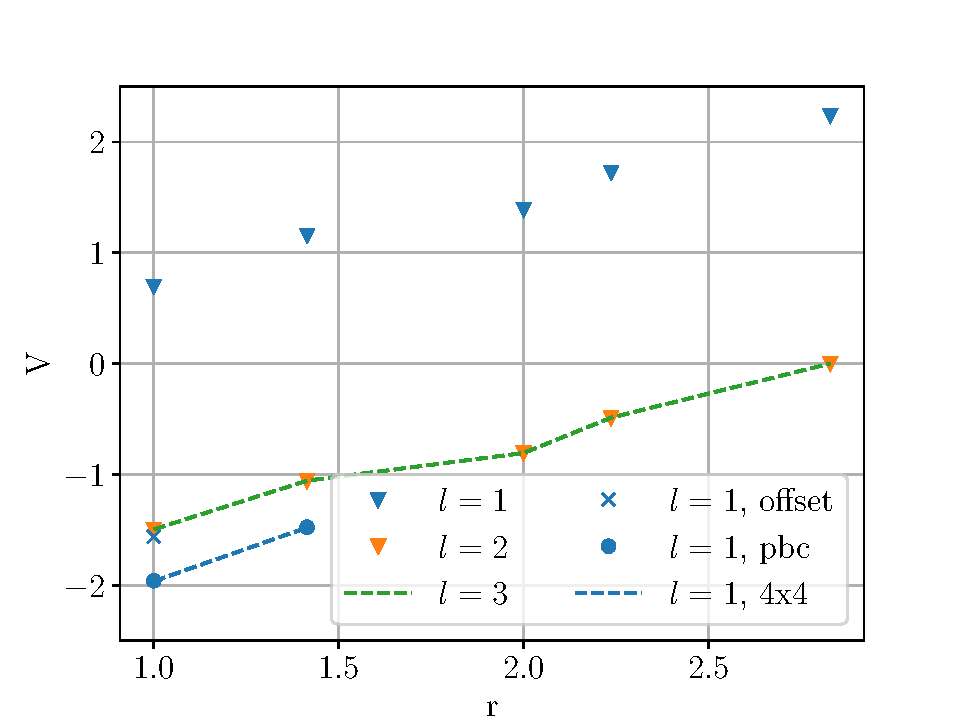
\includegraphics[width=0.45\textwidth]{images/quark_antiquark_potential_large_g.pdf}
	\end{center}
  \caption{Quark-Antiquark potential for diffrent but comparable setups at $g=\num{1.2}$. By default $3\cross3$ dimensions and no PBC, if not stated otherwise.}\label{fig:qqbarl}
\end{figure}
We see, that the potential is not so linear any more and begins to form steps, which shows that for large coupling the lattice fragments are intensified.
We also see a larger seperation of the truncation $l=2$ and $l=3$ in respect to $l=1$. Furthermore the potential of the $4\cross4$ lattice or the $3\cross3$ lattice with PBC is unchanged. It seems as if the truncation gains importains for larger couplings, where as the lattice size keeps its importance as is. Interestingly the potential for the centered charge pair ($l=1$, offset) moves with the $l=2$ and $l=3$ truncated potentials.

Second we compute $g=0.8$ and get \cref{fig:qqbars}.
\begin{figure}[h]
	\begin{center}
		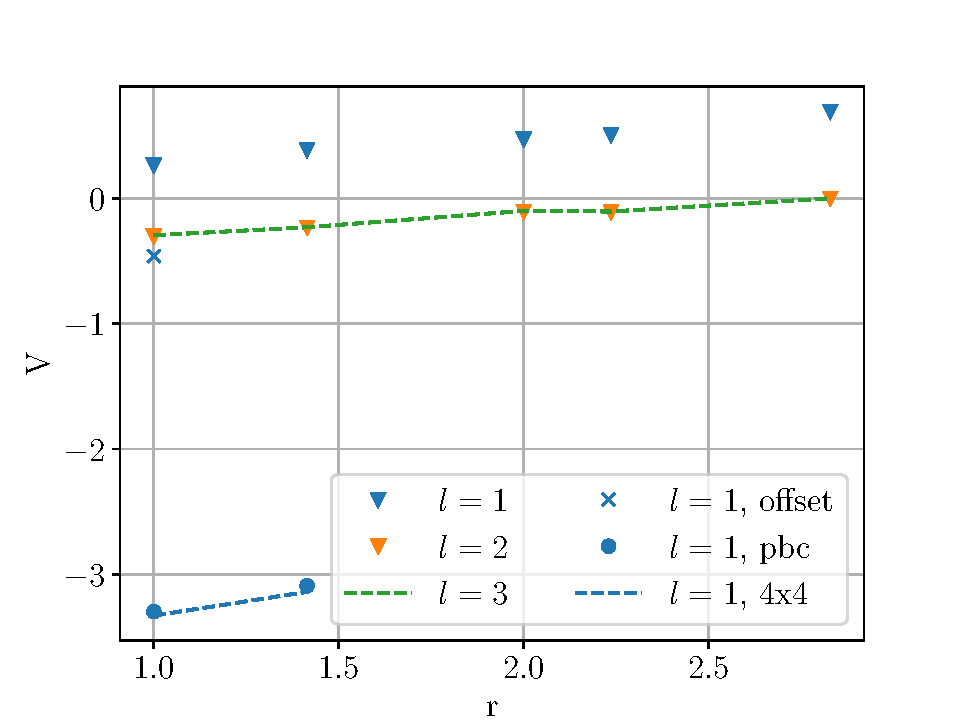
\includegraphics[width=0.45\textwidth]{images/quark_antiquark_potential_small_g.pdf}
	\end{center}
  \caption{Quark-Antiquark potential for diffrent but comparable setups at $g=\num{0.8}$. By default $3\cross3$ dimensions and no PBC, if not stated otherwise.}\label{fig:qqbars}
\end{figure}
Here the $l=2$ and $l=3$ truncated potentials decrease in seperation in respect to the $l=1$ truncated potential. The potential for the $4\cross 4$ and the $3\cross3$ lattice with PBC start to increase in seperatin in respect to the $3\cross3$ lattice with PBC and truncation $l=1$. This indicates, that as the coupling decreases the truncation looses in importance and the lattice volume, i.e. the number of total links, increases. The potential with the centered charge pair moves just as with large couplings with the truncation of $l=2$ and $l=3$. This shows, that not the fact, that no charge is placed on the rim is important, but the actual lattice volume.


% TODO: A $3\cross3$ lattice with $l=2$ and PBC has \num{1.9e6} physical states and takes about an hour. A $5\cross 5$ lattice with $l=1$ and no PBC has \num{}


\iffalse
	\subsection{Step scaling}
	\begin{figure}[h]
		\begin{center}
			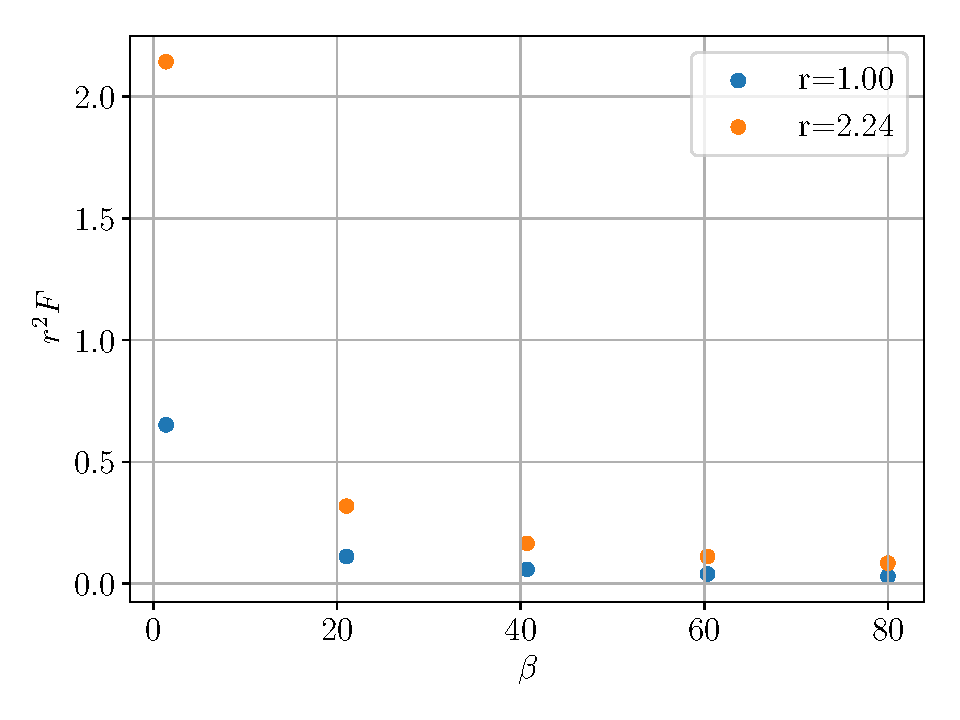
\includegraphics[width=0.45\textwidth]{images/step_scaling.pdf}
		\end{center}
		\caption{Step scaling}
	\end{figure}
\fi
